% Options for packages loaded elsewhere
\PassOptionsToPackage{unicode}{hyperref}
\PassOptionsToPackage{hyphens}{url}
%
\documentclass[
]{article}
\usepackage{amsmath,amssymb}
\usepackage{lmodern}
\usepackage{iftex}
\ifPDFTeX
  \usepackage[T1]{fontenc}
  \usepackage[utf8]{inputenc}
  \usepackage{textcomp} % provide euro and other symbols
\else % if luatex or xetex
  \usepackage{unicode-math}
  \defaultfontfeatures{Scale=MatchLowercase}
  \defaultfontfeatures[\rmfamily]{Ligatures=TeX,Scale=1}
\fi
% Use upquote if available, for straight quotes in verbatim environments
\IfFileExists{upquote.sty}{\usepackage{upquote}}{}
\IfFileExists{microtype.sty}{% use microtype if available
  \usepackage[]{microtype}
  \UseMicrotypeSet[protrusion]{basicmath} % disable protrusion for tt fonts
}{}
\makeatletter
\@ifundefined{KOMAClassName}{% if non-KOMA class
  \IfFileExists{parskip.sty}{%
    \usepackage{parskip}
  }{% else
    \setlength{\parindent}{0pt}
    \setlength{\parskip}{6pt plus 2pt minus 1pt}}
}{% if KOMA class
  \KOMAoptions{parskip=half}}
\makeatother
\usepackage{xcolor}
\usepackage[margin=1in]{geometry}
\usepackage{longtable,booktabs,array}
\usepackage{calc} % for calculating minipage widths
% Correct order of tables after \paragraph or \subparagraph
\usepackage{etoolbox}
\makeatletter
\patchcmd\longtable{\par}{\if@noskipsec\mbox{}\fi\par}{}{}
\makeatother
% Allow footnotes in longtable head/foot
\IfFileExists{footnotehyper.sty}{\usepackage{footnotehyper}}{\usepackage{footnote}}
\makesavenoteenv{longtable}
\usepackage{graphicx}
\makeatletter
\def\maxwidth{\ifdim\Gin@nat@width>\linewidth\linewidth\else\Gin@nat@width\fi}
\def\maxheight{\ifdim\Gin@nat@height>\textheight\textheight\else\Gin@nat@height\fi}
\makeatother
% Scale images if necessary, so that they will not overflow the page
% margins by default, and it is still possible to overwrite the defaults
% using explicit options in \includegraphics[width, height, ...]{}
\setkeys{Gin}{width=\maxwidth,height=\maxheight,keepaspectratio}
% Set default figure placement to htbp
\makeatletter
\def\fps@figure{htbp}
\makeatother
\setlength{\emergencystretch}{3em} % prevent overfull lines
\providecommand{\tightlist}{%
  \setlength{\itemsep}{0pt}\setlength{\parskip}{0pt}}
\setcounter{secnumdepth}{5}
\newlength{\cslhangindent}
\setlength{\cslhangindent}{1.5em}
\newlength{\csllabelwidth}
\setlength{\csllabelwidth}{3em}
\newlength{\cslentryspacingunit} % times entry-spacing
\setlength{\cslentryspacingunit}{\parskip}
\newenvironment{CSLReferences}[2] % #1 hanging-ident, #2 entry spacing
 {% don't indent paragraphs
  \setlength{\parindent}{0pt}
  % turn on hanging indent if param 1 is 1
  \ifodd #1
  \let\oldpar\par
  \def\par{\hangindent=\cslhangindent\oldpar}
  \fi
  % set entry spacing
  \setlength{\parskip}{#2\cslentryspacingunit}
 }%
 {}
\usepackage{calc}
\newcommand{\CSLBlock}[1]{#1\hfill\break}
\newcommand{\CSLLeftMargin}[1]{\parbox[t]{\csllabelwidth}{#1}}
\newcommand{\CSLRightInline}[1]{\parbox[t]{\linewidth - \csllabelwidth}{#1}\break}
\newcommand{\CSLIndent}[1]{\hspace{\cslhangindent}#1}
\usepackage{float}
\ifLuaTeX
  \usepackage{selnolig}  % disable illegal ligatures
\fi
\IfFileExists{bookmark.sty}{\usepackage{bookmark}}{\usepackage{hyperref}}
\IfFileExists{xurl.sty}{\usepackage{xurl}}{} % add URL line breaks if available
\urlstyle{same} % disable monospaced font for URLs
\hypersetup{
  pdftitle={HUX2021 / Dokumentation},
  pdfauthor={St.~Schwarz},
  hidelinks,
  pdfcreator={LaTeX via pandoc}}

\title{HUX2021 / Dokumentation}
\usepackage{etoolbox}
\makeatletter
\providecommand{\subtitle}[1]{% add subtitle to \maketitle
  \apptocmd{\@title}{\par {\large #1 \par}}{}{}
}
\makeatother
\subtitle{HA Empirische Methoden der Sprachwissenschaft / Meinschäfer/Schirakowski SS20 FUB}
\author{St.~Schwarz}
\date{2023-06-11}

\begin{document}
\maketitle

{
\setcounter{tocdepth}{2}
\tableofcontents
}
\begin{longtable}[]{@{}l@{}}
\toprule()
\endhead
to self compile the RMarkdown source to this document in RStudio cf.~\href{https://github.com/esteeschwarz/DH_essais/blob/main/sections/hux2021/rmd/hux_ha_main.Rmd}{Schwarz (2021)} \\
\bottomrule()
\end{longtable}

\hypertarget{draft-abstract}{%
\section{draft abstract}\label{draft-abstract}}

Ich werde in dieser Arbeit den Versuch unternehmen, ein im Rahmen empirischer Studien durchgeführtes \href{https://github.com/esteeschwarz/essais/docs/hux2021}{psycholinguistisches Experiment} ausführlich zu dokumentieren. Die Studie wurde in einem Forschungsseminar der BUA\footnote{Berlin University Alliance} in Kooperation Studierender von FU, TU, HU unter der Aufsicht der Charite durchgeführt. Es handelt sich in diesem Teil um die partielle Replikation des von Paula Rubio-Fernandez (Rubio-Fernández, Cummins, and Tian 2016) unternommenen Versuchs, das Metaphernverständnis von schizophrenen Personen zu untersuchen. Dazu wurde in der Kontrollgruppe ein \emph{self paced reading} Experiment veranstaltet und ausgewertet.

\hypertarget{zum-experiment}{%
\section{Zum Experiment}\label{zum-experiment}}

Das Experiment hat in einer Laufzeit von zwei Wochen Daten von 46 Versuchspersonen erhoben, die hauptsächlich in der Statistiksprache R ausgewertet wurden. Basis der Daten ist die Messung von Lesezeiten in einem set von 24 items\footnote{\emph{item} hier als ein in vier Ausprägungen entworfener Text mit durchschnittlicher Länge von 0 Zeichen.}, die in vierfacher Ausprägung literale und figurative Elemente in kurzen Zusammenhängen verbanden.

\hypertarget{theorierahmen}{%
\section{Theorierahmen}\label{theorierahmen}}

Mit Carston (Carston 2010) sind wir davon ausgegangen, dasz im Experiment zu untersuchende \emph{single} (SM = Metapher eingebettet in literalen Kontext) und \emph{extended metaphors} (EM = erweiterte Metapher, eingebettet in weitgehend figurativen Kontext) unterschiedlich verarbeitet werden, wobei durch die notwendige Aktivierung und Reaktivierung der literalen Bedeutung (ad hoc concept) an SM ein höherer Aufwand nötig sei, der im Gegensatz zu EM in einer längeren Lesezeit resultiert. Diese Annahme führt zu folgenden Fragestellungen, die in Anlehnung an ein Experiment (Verifikation/Replikation) von Paula Rubio-Fernandez et al. (Rubio-Fernández, Cummins, and Tian 2016) hier aufgenommen wurden:

\begin{enumerate}
\def\labelenumi{\arabic{enumi}.}
\tightlist
\item
  unterscheiden sich die Lesezeiten kurzer Texte, die nach den Annahmen folgendem Muster single und extended metaphors enthalten oder rein literal (LC) aufgebaut sind?\\
\item
  wie unterscheidet sich eine vierte Variante, bei der die Struktur der SM invertiert wurde (ISM = literales Element eingebettet in weitgehend figurativen Kontext), hinsichtlich ihrer Verarbeitungszeit?
\end{enumerate}

Die zu überprüfenden Hypothesen lauten wie folgt:

\begin{enumerate}
\def\labelenumi{\arabic{enumi}.}
\tightlist
\item
  Lesezeit SM \textgreater{} Lesezeit EM\\
\item
  Lesezeit EM = Lesezeit LC\\
\item
  Lesezeit ISM = SM \textgreater{} EM = LC
\end{enumerate}

Zur Überprüfung der Hypothesen wurde ein \emph{self paced reading} Experiment durchgeführt, das die Lesezeit in den unterschiedlichen Kategorien erfasste.

\hypertarget{dokumentation}{%
\section{Dokumentation}\label{dokumentation}}

Ich werde im Folgenden den Aufbau und Ablauf des Experiments erklären und im nächsten Abschnitt dessen hypothesengeleitete Auswertung erläutern.

\hypertarget{design}{%
\subsection{Design}\label{design}}

Die Versuchspersonen bekamen während des Tests, der online über einen link abrufbar war, ein set aus jeweils 8 items (Kontexte) die wiederum die Varianten der Variable (Einbettung der Metapher) in Ausprägungen von

\begin{itemize}
\tightlist
\item
  LC (Metapher literal in literalem Kontext)\\
\item
  SM (Metapher figurativ in literalem Kontext)\\
\item
  EM (Metapher figurativ in figurativem Kontext)\\
\item
  ISM (Metapher literal in figurativem Kontext)
\end{itemize}

enthielten sowie einen Bestand aus 16 filler items, die sich ebenfalls in den Kontextvarianten unterschieden. Die Probandinnen lasen einen Text, von dem jeweils nur eine Zeile nicht maskiert war, die jeweils folgende Zeile wurde durch das Drücken der Leertaste sichtbar. So konnte die Verweildauer auf einer sichtbaren Zeile gemessen werden. Als Grundlage für die Messung wurde ein von (Rose 2022) frei verfügbares javascript benutzt, das an unsere Bedürfnisse angepasst worden war; u.a. war ursprünglich keine dauerhafte Speicherung der Daten in einer Datei vorgesehen, diese Funktion wurde von mir \href{https://github.com/esteeschwarz/essais/tree/main/docs/hux2021/experiment/JESPR_original\%26modified}{mit einigem Aufwand realisiert}, so dasz die Lesezeiten danach in einer Tabelle verfügbar waren.\\
Die Einbettung des Experiments in einen auf der Plattform \href{https://soscisurvey.de}{soscisurvey} als akademische Studie angemeldeten Fragebogen erforderte ebenfalls einigen Aufwand, da die Randomisierung der Itemabfrage in anderer Weise als vom script vorgesehen geschehen muszte.\\
Die Daten selbst enthielten Werte für:

\begin{itemize}
\tightlist
\item
  den Start und Endzeitpunkt des durchgeführten Tests (tnid)\\
\item
  die Position der einzelnen maskierten Phrasen im Satz (targetposition) (unabhängige Variable)\\
\item
  die Verweildauer auf den jeweiligen Positionen (elapsed time) (abhängige Variable)\\
\item
  Angaben über die Zuordnung der Phrasen zur jeweiligen Ausprägung (Kategorie) der unabhängigen Variablen
\end{itemize}

\hypertarget{zum-inhalt-des-tests}{%
\subsection{Zum Inhalt des Tests}\label{zum-inhalt-des-tests}}

Die items, die in Anlehnung an R/F nach obigem Muster von uns entworfen wurden, entsprachen im Aufbau dem set, das R/F in ihrem Test verwendet hatte; vier ihrer im Anhang zur Verfügung gestellten items hatten wir ins deutsche übersetzt und eines davon als item in vier Varianten, die restlichen als filler übernommen. Die Auswahl der verwendeten items wurde gemeinschaftlich nach Kriterien wie Konsistenz innerhalb der items, Stil und Kohärenz bestimmt. Ebenfalls nach den constraints von R/F gerichtete Vorgaben wie Wort- und Phrasenlänge (\texttt{median\ characters/phrase\ =} \texttt{44}), Itemlänge (\texttt{median\ characters/item\ =} \texttt{0}) und Position des targets hatten beim Entwurf eine wichtige Rolle gespielt, waren jedoch nicht immer optimal umgesetzt worden; dazu einige Bemerkungen im Auswertungsteil. Ein item sollte eine Metapher in je figurativer und literaler Bedeutung, eingebettet in einen je figurativen oder literalen Kontext, d.h. also in insgesamt vier unterschiedlichen Konfigurationen, präsentieren. Die Metapher (unser target) sollte sich im dritten Viertel des Kontextes befinden, um davor und danach auftretende Latenzen der Lesezeit auswerten zu können. Dafür wurden im script des Tests die Positionen der einzeln zu lesenden Phrasen des items mit 0 für das target und je negativen und positiven Werten für den Abstand zum target festgelegt.\footnote{da diese Positionen erst :nach: Start des Tests konsequent im script festgelegt wurden, muszte bei der Auswertung einiges manuell nachgearbeitet werden, um die Daten konsistent zu halten.}\\
Das set eines einzelnen durch Abruf des Fragebogens aufgerufenen Tests bestand für jede Studienteilnehmerin aus einer randomisierten Auswahl einer von vier mal acht Itemvarianten (aus der Menge von 8 items), womit jeweils zweifach Meszdaten der vier Varianten pro TN erhoben werden konnten, aber niemals ein TN ein item in mehreren Varianten las.
Die 16 filler items traten innerhalb des sets aus also 24 items an zufälligen Positionen auf, wurden aber bei allen TN aus demselben pool bedient und wiesen ausgeglichene Variation hinsichtlich der figurativ-literalen Konfiguration auf.

\hypertarget{auswertung}{%
\subsection{Auswertung}\label{auswertung}}

O.a. Daten wurden in R (RStudio and PBC 2022) 1. deskriptiv und 2. mittels des Paketes lme4 (Bates et al. 2015) zur Erhebung kovariater Abhängigkeiten (linear mixed model) analog der Vorgaben (Rubio-Fernández, Cummins, and Tian 2016) ausgewertet. Das script dazu kann \href{https://github.com/esteeschwarz/essais/tree/main/docs/hux2021/evaluation}{hier}, sowie eine visualisierte, vom user nach eigenen Parametern anzupassende deskriptive Auswertung \href{https://vision2020.shinyapps.io/hux2021}{hier} nachvollzogen werden. Für eine ausschnitthafte Visualisierung cf.~(Figure @ref(fig:fig-01), @ref(fig:fig-02), @ref(fig:fig-03)).

\hypertarget{a.}{%
\subsubsection{a.}\label{a.}}

Zur Auswertung wurden die erhobenen durch ein php-script im flachen comma-separated Format gespeicherten Lesezeiten in R importiert. Um zu gewährleisten, dasz Abweichungen hinsichtlich der Zeichenanzahl der zeitgemessenen Phrasen keine unerwünschten Effekte in der Berechnung der Latenzen zeitigen, wurde bei jeder weiteren Berechnung dafür ein von der Zeichenanzahl/Phrase anhängiger Koeffizient einbezogen, der in der ersten, deskriptiven Auswertung einfach aus der Zeichenanzahl, bei der zweiten kovariaten Auswertung mittels lme4 bestimmt (Fine et al. 2013) und als Residual (hier: korrigierte Lesezeit) einbezogen wurde. R/F hatten ihre Daten mit dem R-package lme4 unter multivariaten Gesichtspunkten analysiert; so konnte auch ich (in dieser Phase ging die Experiment-Arbeitsgruppe getrennte Wege) nach Feststellung des Effekts der Phrasenlänge und Berücksichtigung desselben als korrigierte Lesezeit (hier: die abhängige Variable in der lmer Formel) signifikante Unterschiede der Lesezeiten von ISM und LC feststellen. Allerdings nur an dieser Stelle, womit einzelne Hypothesen nicht bestätigt werden konnten. Bei der Multivarianzanalyse wurden hier ein \emph{main effect} der Kategorie (LC, SM, EM, ISM = group) unter \emph{random effects} von TN (participant) und Kategorie auf TN (group by participant) vorausgesetzt.

\hypertarget{b.}{%
\subsubsection{b.}\label{b.}}

Deskriptiv konnten am target keine signifikanten Unterschiede in der durchschnittlichen Lesezeit an den verschieden eingebetteten Metaphern festgestellt werden. Da mir noch wesentliche Grundlagen zur Interpretation der Ergebnisse der Multivarianzanalyse fehlen und es sich hier nur um die kurze Dokumentation des Experiments im Seminarkontext handeln soll, die endlich abgeschlossen werden soll, werde ich darauf verzichten, meine Ergebnisse der multivariaten Berechnungen zur Grundlage einer dadurch ansatzweise bestätigten 3. Hypothese (ISM \textgreater{} LC) zu stilisieren.

\hypertarget{c.}{%
\subsubsection{c.}\label{c.}}

Grob liesze sich durch die allein deskriptive Auswertung die Aussage machen, dasz sich bei target = -1, 0, 1, Vernachlässigung ungültiger Fälle = 1, outliers discarded = 1 \& korrigierter RT (selection = -1, 0, 1, 1, 1, 0) folgende Hierarchie der Lesezeiten ergibt:\\
EM \textless{} SM \textless{} ISM \textless{} LC. Dabei gilt es zu beachten, dasz der hier gröszte Unterschied der zwischen EM und LC mit 416ms zu messen ist, übersetzt unterhalb einer halben Sekunde liegt. (Zum Vergleich: ein ununterbrochenes Weiterklicken der lesbaren Zeilen mittels der space-Taste zeigt ca. 200ms Latenz.)\\
Siehe dazu den Ausschnitt \texttt{TI\ +\ rtc} = length corrected reading time

\begin{tabular}{l|l|l|r|r|r|r|r}
\hline
  & RT & group & LZ & dif\_SM & dif\_EM & dif\_LC & dif\_ISM\\
\hline
6 & TI + rtc & EM & 1927 & -10 & NA & -416 & -389\\
\hline
5 & TI + rtc & SM & 1937 & NA & 10 & -406 & -379\\
\hline
8 & TI + rtc & ISM & 2316 & 379 & 389 & -27 & NA\\
\hline
7 & TI + rtc & LC & 2343 & 406 & 416 & NA & 27\\
\hline
\end{tabular}

aus der folgenden Tabelle:\footnote{Für weitere Ansichten und Studiensample besuchen Sie bitte \href{https://vision2020.shinyapps.io/hux2021}{o.a. interaktive Visualisierungen}.}

\begin{tabular}{l|l|r|r|r|r|r}
\hline
RT & group & LZ & dif\_SM & dif\_EM & dif\_LC & dif\_ISM\\
\hline
TimeInterval & SM & 2256 & NA & 117 & -242 & -190\\
\hline
TimeInterval & EM & 2139 & -117 & NA & -359 & -307\\
\hline
TimeInterval & LC & 2499 & 242 & 359 & NA & 53\\
\hline
TimeInterval & ISM & 2446 & 190 & 307 & -53 & NA\\
\hline
TI + rtc & SM & 1937 & NA & 10 & -406 & -379\\
\hline
TI + rtc & EM & 1927 & -10 & NA & -416 & -389\\
\hline
TI + rtc & LC & 2343 & 406 & 416 & NA & 27\\
\hline
TI + rtc & ISM & 2316 & 379 & 389 & -27 & NA\\
\hline
TI char & SM & 2449 & NA & 4 & -2 & -24\\
\hline
TI char & EM & 2445 & -4 & NA & -6 & -27\\
\hline
TI char & LC & 2451 & 2 & 6 & NA & -22\\
\hline
TI char & ISM & 2473 & 24 & 27 & 22 & NA\\
\hline
\end{tabular}

Bei isoliertem target (target = 0, 0, 0) ergibt sich folgende Hierarchie der Lesezeiten:\\
EM \textless{} SM \textless{} LC \textless{} ISM mit dem gröszten Unterschied zwischen EM und ISM mit 400ms.

\begin{tabular}{l|l|l|r|r|r|r|r}
\hline
  & RT & group & LZ & dif\_SM & dif\_EM & dif\_LC & dif\_ISM\\
\hline
6 & TI + rtc & EM & 1388 & -157 & NA & -364 & -400\\
\hline
5 & TI + rtc & SM & 1545 & NA & 157 & -207 & -243\\
\hline
7 & TI + rtc & LC & 1753 & 207 & 364 & NA & -36\\
\hline
8 & TI + rtc & ISM & 1788 & 243 & 400 & 36 & NA\\
\hline
\end{tabular}

\textbf{\emph{LEGENDE}}

\begin{itemize}
\tightlist
\item
  \textbf{LZ:} berechnete Lesezeit (response time)
\item
  \textbf{TimeInterval:} uncorrected response time (TI)\\
\item
  \textbf{TI + RTC:} TimeInterval + lmer residuals of TI dependent on phrase length\\
\item
  \textbf{TI char:} TimeInterval corrected by mean phrase length (TI/characters*mean(characters))
\end{itemize}

\begin{figure}[H]
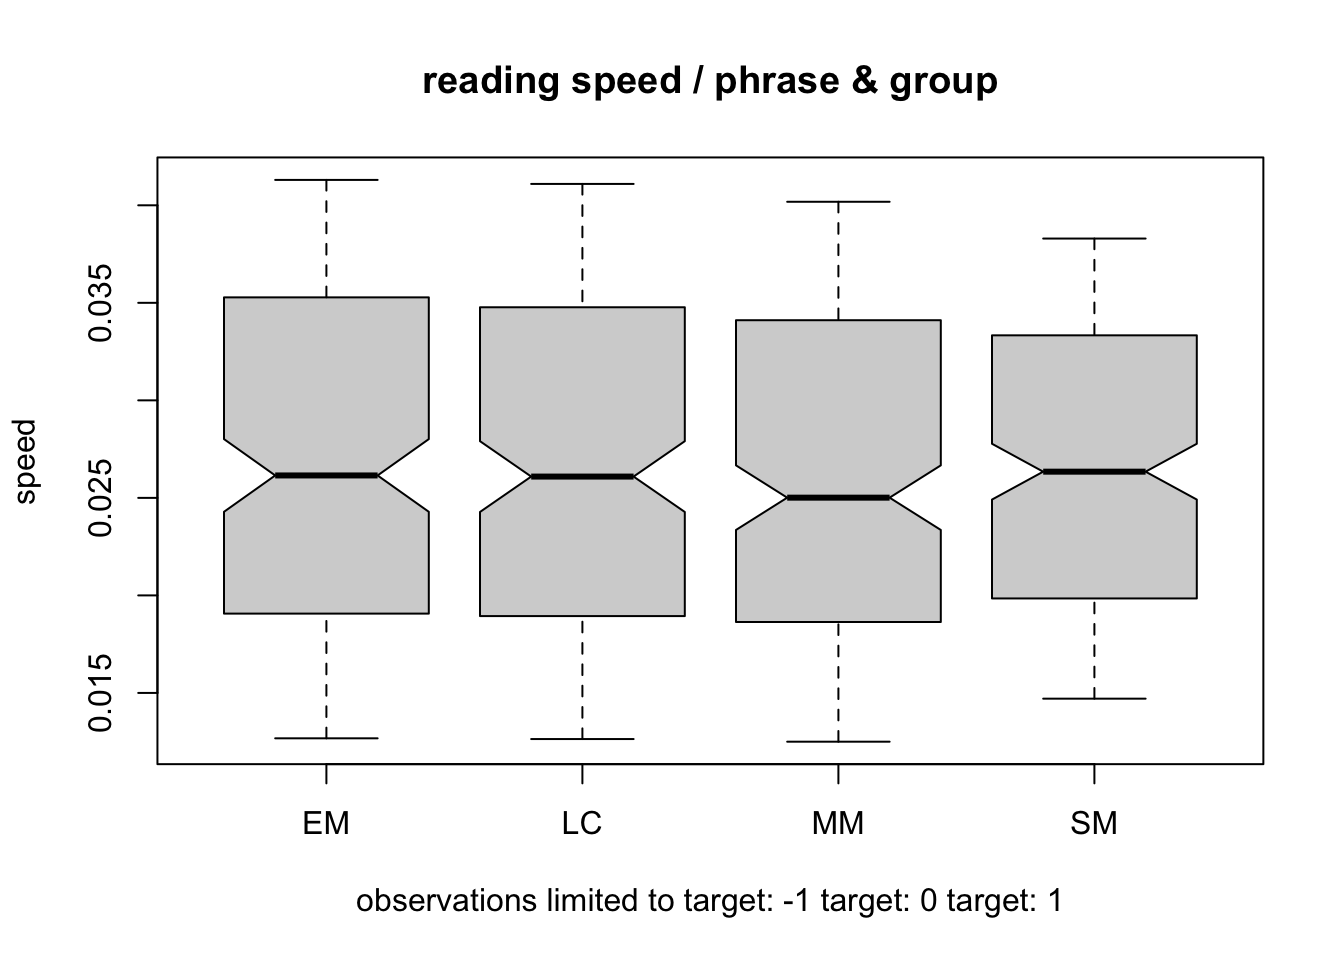
\includegraphics{/Users/guhl/Documents/GitHub/DH_essais/sections/hux2021/hux_HA/pdf/hux_ha_main/hux_ha_main_files/figure-latex/fig-01-1} \caption{evaluate target, target-preceding, target-following phrase, not length corrected}(\#fig:fig-01)
\end{figure}

(\#fig:fig-02)reading times (uncorrected = timeinterval) \& with 2 different approaches of processing the phrase length

\begin{figure}[H]
\includegraphics{/Users/guhl/Documents/GitHub/DH_essais/sections/hux2021/hux_HA/pdf/hux_ha_main/hux_ha_main_files/figure-latex/fig-02-2} \caption{reading times (uncorrected = timeinterval) & with 2 different approaches of processing the phrase length}(\#fig:fig-02)
\end{figure}

(\#fig:fig-03)comparing SM vs.~other

\begin{figure}[H]
\includegraphics{/Users/guhl/Documents/GitHub/DH_essais/sections/hux2021/hux_HA/pdf/hux_ha_main/hux_ha_main_files/figure-latex/fig-03-2} \caption{comparing SM vs. other}(\#fig:fig-03)
\end{figure}

\begin{center}\rule{0.5\linewidth}{0.5pt}\end{center}

\hypertarget{b.-ref}{%
\section*{B. REF:}\label{b.-ref}}
\addcontentsline{toc}{section}{B. REF:}

\hypertarget{refs}{}
\begin{CSLReferences}{1}{0}
\leavevmode\vadjust pre{\hypertarget{ref-bates_fitting_2015}{}}%
Bates, Douglas, Martin Mächler, Ben Bolker, and Steve Walker. 2015. {``Fitting {Linear} {Mixed}-{Effects} {Models} {Using} Lme4.''} \emph{Journal of Statistical Software} 67 (1): 1--48. \url{https://doi.org/10.18637/jss.v067.i01}.

\leavevmode\vadjust pre{\hypertarget{ref-carston_xiii-metaphor_2010}{}}%
Carston, Robyn. 2010. {``{XIII}-{Metaphor}: {Ad} {Hoc} {Concepts}, {Literal} {Meaning} and {Mental} {Images}.''} \emph{Proceedings of the Aristotelian Society} 110 (3pt3): 295--321. \url{https://doi.org/10.1111/j.1467-9264.2010.00288.x}.

\leavevmode\vadjust pre{\hypertarget{ref-fine_rapid_2013}{}}%
Fine, Alex B., T. Florian Jaeger, Thomas A. Farmer, and Ting Qian. 2013. {``Rapid {Expectation} {Adaptation} During {Syntactic} {Comprehension}.''} \emph{PLOS ONE} 8 (10): e77661. \url{https://doi.org/10.1371/journal.pone.0077661}.

\leavevmode\vadjust pre{\hypertarget{ref-rose_jespr_2022}{}}%
Rose, Ralph. 2022. {``{JESPR}.''} \url{https://github.com/fildpauz/jespr}.

\leavevmode\vadjust pre{\hypertarget{ref-rstudio_rstudio_2022}{}}%
RStudio, and PBC. 2022. {``{RStudio} {IDE}.''} \url{https://www.rstudio.com/products/rstudio/download/}.

\leavevmode\vadjust pre{\hypertarget{ref-rubio-fernandez_are_2016}{}}%
Rubio-Fernández, Paula, Chris Cummins, and Ye Tian. 2016. {``Are Single and Extended Metaphors Processed Differently? {A} Test of Two {Relevance}-{Theoretic} Accounts.''} \emph{Journal of Pragmatics} 94 (March): 15--28. \url{https://doi.org/10.1016/j.pragma.2016.01.005}.

\leavevmode\vadjust pre{\hypertarget{ref-schwarz_rmarkdown_2021}{}}%
Schwarz, St. 2021. {``{RMarkdown} Source to This Document.''} \url{https://github.com/esteeschwarz/DH_essais/blob/main/sections/hux2021/hux_HA/hux_ha_main.Rmd}.

\end{CSLReferences}

\end{document}
